\section{Three Address Code}
We chose to implement the indirect triples approach to represent internally
the three address code. As stated in the Dragon Book \cite{dragonbook} this 
representation
can help in optimizing the resulting code, because the instructions can be
easily swapped to improve the performances.

We generate the three address code from an AST, that passed the type checking
phase. To make it even easier to deal the instructions we chose to use
doubly-linked lists.

The following F code is represented in 3AC as depicted in Fig. 
\ref{fig:ind-trpl}:
\begin{verbatim}
fract a = [1|1];
fract b = [1|3] * a + [1|2];
\end{verbatim}

While traversing the AST we generate the three address code in a bottom up
fashion using \emph{only} synthesized attributes. This makes the three address
code generator intuitive.

\begin{figure}[H]
  \centering
  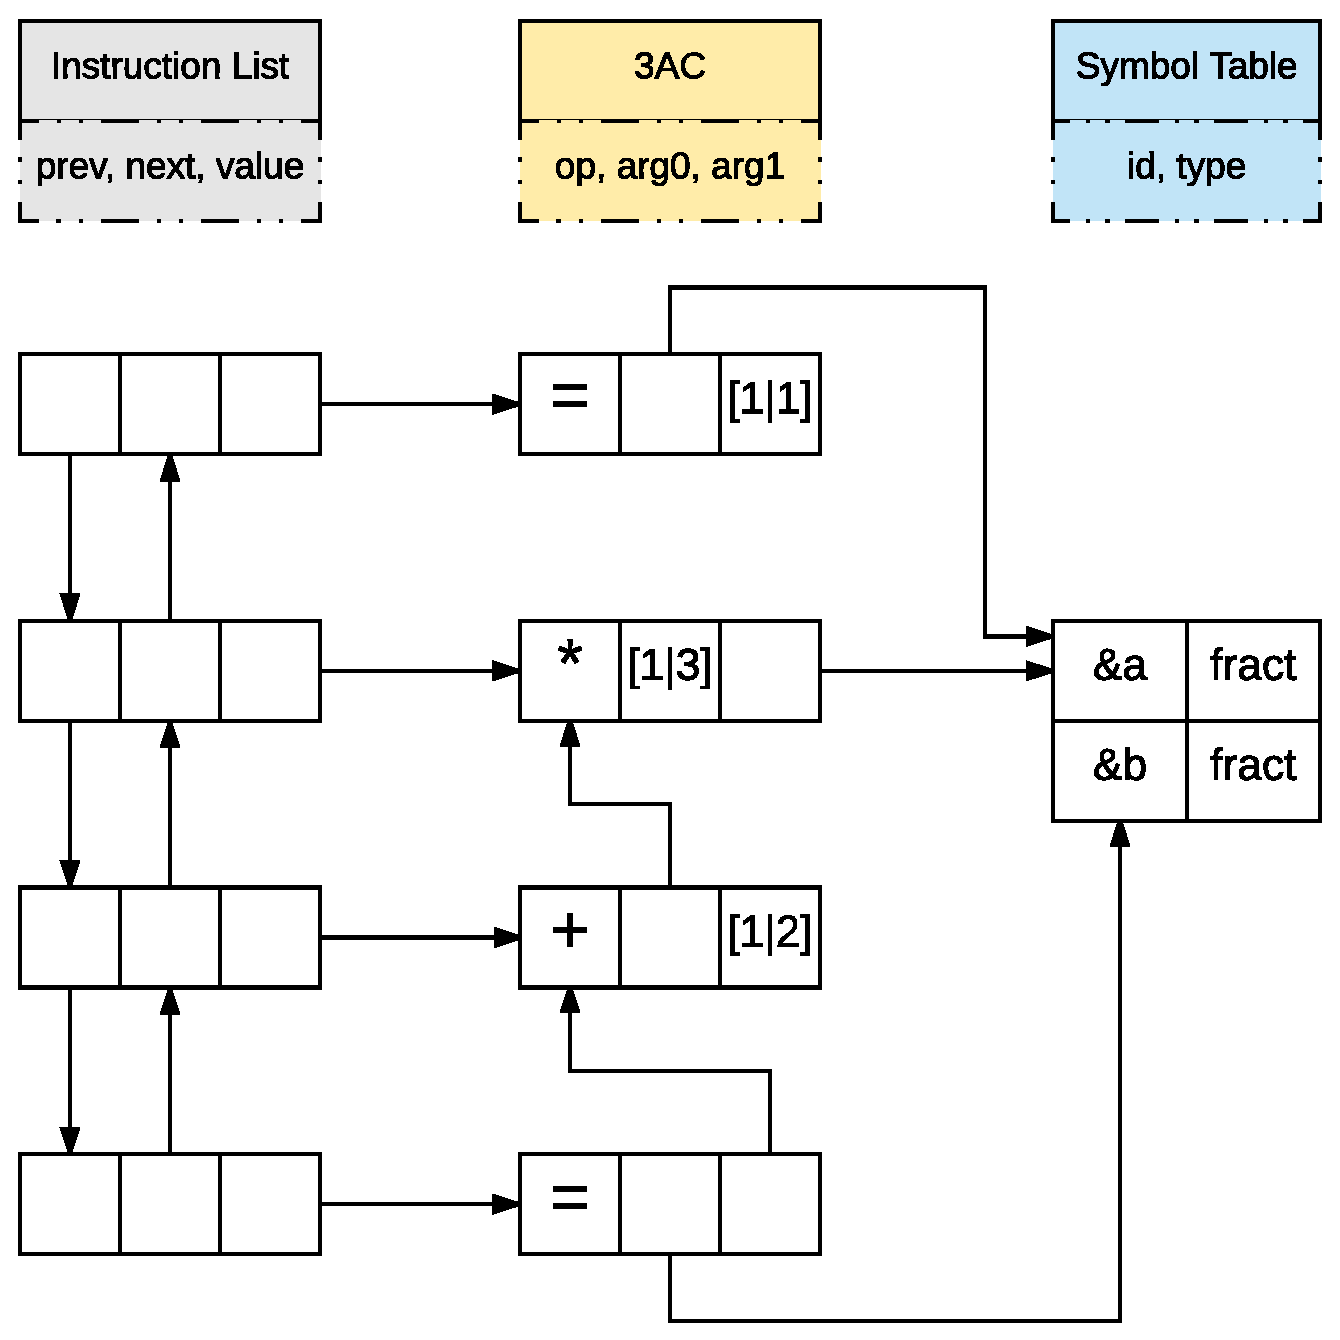
\includegraphics[width=.9\columnwidth]{img/eps/indirect_triples.eps}
  \caption{FAC - example of indirected triples.}
  \label{fig:ind-trpl}
\end{figure}
